\pdfbookmark{Общая характеристика работы}{characteristic}             % Закладка pdf
\begin{center}
    \section*{ОБЩАЯ ХАРАКТЕРИСТИКА РАБОТЫ}
\end{center}

\newcommand{\actuality}{\pdfbookmark[1]{Актуальность}{actuality}\underline{\textbf{\actualityTXT}}}
\newcommand{\progress}{\pdfbookmark[1]{Разработанность темы}{progress}\underline{\textbf{\progressTXT}}}
\newcommand{\aim}{\pdfbookmark[1]{Цели}{aim}\underline{{\textbf\aimTXT}}}
\newcommand{\tasks}{\pdfbookmark[1]{Задачи}{tasks}\underline{\textbf{\tasksTXT}}}
\newcommand{\aimtasks}{\pdfbookmark[1]{Цели и задачи}{aimtasks}\aimtasksTXT}
\newcommand{\novelty}{\pdfbookmark[1]{Научная новизна}{novelty}\underline{\textbf{\noveltyTXT}}}
\newcommand{\influence}{\pdfbookmark[1]{Практическая значимость}{influence}\underline{\textbf{\influenceTXT}}}
\newcommand{\methods}{\pdfbookmark[1]{Методология и методы исследования}{methods}\underline{\textbf{\methodsTXT}}}
\newcommand{\defpositions}{\pdfbookmark[1]{Положения, выносимые на защиту}{defpositions}\underline{\textbf{\defpositionsTXT}}}
\newcommand{\reliability}{\pdfbookmark[1]{Достоверность}{reliability}\underline{\textbf{\reliabilityTXT}}}
\newcommand{\probation}{\pdfbookmark[1]{Апробация}{probation}\underline{\textbf{\probationTXT}}}
\newcommand{\contribution}{\pdfbookmark[1]{Личный вклад}{contribution}\underline{\textbf{\contributionTXT}}}
\newcommand{\publications}{\pdfbookmark[1]{Публикации}{publications}\underline{\textbf{\publicationsTXT}}}


{\actuality} В условиях растущего мирового населения и активной глобальной индустриализации, сопровождаемых повышением объемов потребления электроэнергии,
все более актуальной становится \fixme{разработка новых подходов и источников энергии}, способных обеспечить устойчивое и надежное энергоснабжение. \fixme{Необходимость в этом также обуславливается стремлением к эффективному использованию природных ресурсов и минимизации негативного воздействия на окружающую среду.} Одним из наиболее перспективных направлений является управляемый термоядерный синтез (УТС), рассматриваемый в качестве \fixme{<<чистой>> альтернативы традиционным подходам на основе сжигания ископаемых ресурсов, так и ключевого звена гибридной системы в реакторах типа синтез-деление.} Прогресс в области УТС может стать ключевым фактором в развитии энергетических технологий следующего поколения.

За последние десятилетия наибольшие успехи на пути к практической реализации контролируемой реакции УТС были достигнуты в установках с магнитным удержанием горячей плазмы типа токамак. Возможность \fixme{горения} дейтерий-тритиевой (DT) реакции термоядерного синтеза была продемонстрирована на токамаках TFTR~\cite{Skinner1997} и JET~\cite{Keilhacker1999} еще в конце XX века. Последующая модернизация токамака JET и оптимизация методики эксперимента позволила достичь \fixme{на сегодняшний день рекордных параметров DT-плазмы с протекающей реакцией синтеза и длительностью разряда около \SI{6}{\second}}~\cite{Maggi2024,Kappatou2025}. На токамаках WEST и EAST были получены рекордные результаты по длительности удержания горячей плазмы (без генерации термоядерной энергии) продолжительностью в \(\SI{364}{\second}\)~\cite{Shi2025} и \(\SI{1056}{\second}\)~\cite{Gong2024}, соответственно. Наблюдаемые достижения свидетельствует о перспективности и потенциальной реализуемости УТС за счет удержания термоядерной плазмы в магнитной конфигурации токамака.

В настоящее время идет активная фаза строительства международного экспериментального термоядерного реактора ИТЭР, спроектированного для практической демонстрации возможности \fixme{длительного (\SI{400}{\second})} удержания термоядерной DT-плазмы и решения сопутствующих инженерных задач. Введены в эксплуатацию наибольший в России токамак Т15-МД~\cite{Velikhov2024} и наибольший в мире токамак JT60-SA~\cite{Shirai2024}, расположенный в Японии. Во множестве стран разрабатываются проекты установок следующего поколения для отработки реакторных технологий, в том числе в России ведется активное проектирование токамака с реакторными технологиями (ТРТ)~\cite{Krasilnikov2021}. Помимо этого, растет число частных компаний в области УТС, развивающих уникальные подходы и технологии для коммерческих целей. По данным Ассоциации термоядерной промышленности (FIA)~\cite{FIA}, более 50\% компаний из данной сферы разрабатывают подходы на основе магнитного удержания плазмы, что дополнительно подчеркивает актуальность направления.

Ввод в эксплуатацию термоядерных установок (ТЯУ) потребует решения целого ряда физических и технологических задач. Одними из наиболее существенных остаются проблемы удержания энергии и частиц, выбора материалов обращенных к плазме элементов (ОПЭ), эффективной организации топливного цикла, а также обеспечения радиационной безопасности. Последний пункт обусловлен планируемым использованием смеси дейтерия и радиоактивного трития в качестве топлива для термоядерных реакторов, что определяет необходимость в понимании процессов накопления и систематическом контроле содержания изотопов водорода в конструкционных элементах.

В первых экспериментах с DT-плазмой на токамаках TFTR и JET наблюдалось чрезмерно большое накопление трития~\cite{Gasparyan2024}, связанное с особенностями взаимодействия изотопов водорода с используемыми на тот момент углеродными ОПЭ. Последующие результаты, полученные на токамаках с металлической облицовкой (JET~\cite{Maggi2024,Kappatou2025}: бериллиевая первая стенка и вольфрамовый дивертор; ASDEX-Upgrade~\cite{Rohde2009}: вольфрамовые первая стенка и дивертор), продемонстрировали перспективу в достижении \fixme{соизмеримых} параметров удержания плазмы при одновременном снижении (по сравнению с углеродными ОПЭ) скорости накопления изотопов водорода более чем на порядок. Важно заметить, что вольфрам используется в качестве основного материала наиболее нагруженной области большинства действующих токамаков "--- дивертора. Как материал ОПЭ, вольфрам характеризуется низким коэффициентом распыления легкими ионами и высокой температуростойкости, что может играть ключевую роль в обеспечении продолжительного срока службы под воздействием интенсивных нейтронных и плазменных потоков~\cite{Neu2005}. К тому же, Международной организацией ИТЭР было принято решение о переходе к полностью вольфрамовой облицовке~\cite{Barabaschi2025}, а во множестве проектов демонстрационных реакторов вольфрам рассматривается как приоритетный материал ОПЭ~\cite{Bachmann2016}.

Оценки уровня накопленного трития в ИТЭР~\cite{Roth1,Pitts2025} с полностью вольфрамовой стенкой показывают, что допустимый уровень содержания не должен быть превышен за период эксплуатации. Однако при получении данных консервативных оценок не учитывался ряд процессов, протекание которых ожидается во время работы реактора. Одним из таких факторов являются быстрые переходные процессы, как локализованные на периферии неустойчивости (ELMs "--- Edge localised modes), наблюдаемые в режимах с наилучшими параметрами удержания плазмы в токамаках (H-мода). Развитие ELM-неустойчивости сопровождается \fixme{мощными кратковременными ($\leq\SI{1}{\milli\second}$) потоками тепла и высокоэнергетичных частиц, приходящими на ОПЭ с характерной частотой \(\sim \SIrange{10}{100}{\hertz}\)}. Длительное импульсно-периодическое воздействие плазменных потоков может влиять как на динамику накопления рабочего газа в ОПЭ, так и на процессы взаимодействия плазмы с их поверхностью.

\fixme{Немногочисленные эксперименты по имитации воздействия мощных плазменных потоков, соответствующих ELM-событиям, на захват изотопов водорода в вольфраме проводились на линейных плазменных установках~\cite{Nishijima2011,Poskakalov2020,Ogorodnikova}. Полученные результаты указывают на потенциально большую скорость проникновения изотопов водорода вглубь материала при импульсном воздействии по сравнению со случаем стационарного облучения, характерного для нормальных плазменных разрядов, однако не дают однозначной информации о влиянии на скорость интегрального накопления. Помимо этого, параметры облучения в установках такого типа не могут в полной мере воспроизвести условия, соответствующие крупным токамакам масштаба ИТЭР. Численное моделирование длительного накопления на больших временных масштабах также затруднительно ввиду малой длительности переходных процессов. }

\fixme{Диагностика содержания изотопов водородов в ОПЭ является не менее приоритетным вопросом. В настоящее время особое внимание уделяется развитию методов дистанционного контроля, основанных на использовании лазерного излучения. Одним из таких методов является лазерно-индуцированная десорбция (ЛИД), которая основана на нагреве участка исследуемой поверхности лазерным импульсом с последующим анализом состава вышедшего газа. Применимость ЛИД была продемонстрирована на \fixme{ряде} установок (TEXTOR~\cite{Schweer2009}, JET~\cite{Zlobinski2024}, Глобус-М2~\cite{Medvedev2024} и т.д.), а соответствующие диагностические комплексы разрабатываются для ИТЭР и были предложены для российского проекта ТРТ~\cite{Razdobarin2022}. Выход изотопов водорода из ОПЭ под действием импульсных тепловых нагрузок является схожим и в то же время более простым процессом по сравнению со случаем захвата при импульсно-периодическом плазменном облучении. Тем не менее, исследование основных зависимостей выхода при лазерном нагреве является актуальным вопросом для определения наиболее эффективных режимов диагностического метода.}

{\aim} диссертационной работы является выявление закономерностей процессов удержания и выхода дейтерия в вольфраме при импульсном плазменном и лазерном воздействии.

Для~достижения поставленной цели необходимо было решить следующие~{\tasks}:
\begin{enumerate}[beginpenalty=10000] % https://tex.stackexchange.com/a/476052/104425
    \item \fixme{Построить математическую модель, описывающую транспорт дейтерия в вольфраме под действием импульсных тепловых и плазменных нагрузок.}
    \item \fixme{Провести анализ применимости стандартных моделей транспорта изотопов водорода в материалах к моделированию процессов захвата и десорбции при импульсных нагрузках.}
    \item Оценить параметры плазменных нагрузок, приходящих на ОПЭ во время ELM-событий, \fixme{на основе данных для ИТЭР.}
    \item Исследовать влияние быстрых переходных процессов, соответствующих ELM-событиям, \fixme{на накопление дейтерия в вольфраме на временных масштабах, соответствующих длительности плазменных разрядов в ИТЭР.}
    \item Провести анализ состава потока десорбированного дейтерия с поверхности вольфрама при лазерном нагреве.
    \item \fixme{Определить влияние процессов на поверхности, параметров центров захвата, теплофизических свойств материала и характеристик импульса на выход дейтерия из вольфрама при лазерном нагреве.}
\end{enumerate}

{\methods} Достижение поставленной цели и решение сопутствующих задач осуществлялись путем проведения численного моделирования, которое позволяет исследовать влияние импульсных нагрузок в широком диапазоне параметров, обычно недоступном в рамках действующих экспериментальных и лабораторных установок. Результаты численных расчетов были получены методом конечных элементов в свободно распространяемом программном пакете \href{https://github.com/festim-dev/FESTIM}{FESTIM}, разработанном в международном коллективе при участии автора. Для решения части ресурсоёмких задач были использованы мощности высокопроизводительного вычислительного центра \thesisOrganizationShort. Для демонстрации надежности и корректности использованных моделей проводилась их верификация и валидация путем сравнения с экспериментальными результатами. Построение аналитической модели, описывающей распределение изотопов водорода в вольфраме при наличии центров захвата изотопов водорода и градиента температур (эффект Соре), проводилось путем решения системы дифференциальных уравнений в частных производных методом функции Грина.

{\novelty}
\begin{enumerate}[beginpenalty=10000] % https://tex.stackexchange.com/a/476052/104425
    \item \fixme{Впервые проведено моделирование длительного (\SI{1000}{\second}) накопления дейтерия в вольфрамовых ОПЭ под действием импульсно-периодических плазменных нагрузок, соответствующих ELM-событиям в крупных токамаках, с длительностью одного события \SI{1}{\milli\second} и частотой повторения от \num{10} до \SI{100}{\hertz} (от \num{e4} до \num{e5} событий)}.
    \item \fixme{Предложена оригинальная аналитическая модель, описывающая одномерное стационарное распределение содержания водорода в материалах при наличии центров захвата и градиента температур в приближении мгновенной рекомбинации атомов на обращенной к плазме поверхности и мгновенной рекомбинации или нулевого потока атомов на обратной поверхности.}
    \item Впервые проведен детальный анализ состава потока дейтерия, десорбированного с поверхности вольфрама при лазерном нагреве.
    \item \fixme{Впервые проведена оценка роли процессов на поверхности, центров захвата, теплофизических свойств и параметров импульса на выход дейтерия из поверхностных слоев вольфрама при лазерном нагреве}.
\end{enumerate}

{\influence} заключается в следующем:
\begin{enumerate}[beginpenalty=10000] % https://tex.stackexchange.com/a/476052/104425
    \item \fixme{Результаты анализа влияния импульсно-периодических нагрузок на накопление изотопов водорода в вольфраме могут быть использованы \fixme{для прогноза} содержания изотопов водорода, накопленных в ОПЭ ТЯУ.}
    \item \fixme{Результаты анализа влияния параметров лазерного нагрева и материала на выход дейтерия из поверхностных слоев вольфрама} могут быть использованы при разработке и выборе оптимальных параметров диагностического метода контроля содержания изотопов водорода в ОПЭ, основанного на ЛИД. Результаты экспериментов по ЛИД дейтерия из соосажденных пленок вольфрама могут быть использованы для валидации численных моделей.
    \item Имплементированная в коде FESTIM модель, учитывающая поверхностные процессы, доступна всем пользователям кода и существенно расширяет его область применения. Результаты валидации модели включены в книгу по верификации и валидации кода FESTIM и могут быть использованы для проведения сравнения результатов, полученных с помощью иных кодов.
\end{enumerate}

{\defpositions}
\begin{enumerate}[beginpenalty=10000] % https://tex.stackexchange.com/a/476052/104425
    \item \fixme{Одномерная аналитическая модель, описывающая стационарное распределение водорода в материале при учете центров захвата и градиента температур, позволяет оценить предельное содержание изотопов водорода под действием импульсно-периодических плазменных нагрузок при достижении квазистационарного режима.}
    \item Возникновение импульсно-периодических плазменных нагрузок, соответствующих ELM-событиям в токамаках (частота: 10 "--- 100 Гц, длительность: \SI{1}{\milli\second}, плотность энергии: \SIrange{0.14}{0.45}{\mega\joule\per\meter\squared}), наряду со стационарными плазменными потоками (плотность мощности: \SIrange{1}{10}{\mega\watt\per\meter\squared}) ведет к снижению скорости накопления дейтерия в вольфраме при длительности облучения более \SI{10}{\second} за счет значительного повышения температуры материала относительно случая облучения стационарными потоками плазмы. 
    \item Дополнительный нагрев во время импульсно-периодических плазменных нагрузок, соответствующих ELM-событиям в токамаках, приводит к более быстрому проникновению дейтерия вглубь материала за счет большей подвижности, что может усложнить процесс обезгаживания ОПЭ в ТЯУ. 
    \item \fixme{Атомарная фракции в потоке дейтерия, десорбированного с поверхности вольфрама, растет с увеличением температуры поверхности и уменьшением потока частиц, выходящих на поверхность. Интегральная величина атомарной фракции в потоке десорбированного водорода может достигать $\sim$10~\% при лазерном нагреве с длительностью более \SI{10}{\micro\second} до температуры плавления вольфрама, что может вносить дополнительную погрешность измерений при анализа содержания изотопов водорода методом ЛИД.} 
    \item \fixme{Процессы на поверхности могут приводить к снижению доли десорбированного дейтерия из вольфрама при импульсном лазерном нагреве с длительностью менее \SI{10}{\micro\second}, уменьшая эффективность анализа содержания изотопов водорода в толстых поверхностных слоях методом ЛИД.}
\end{enumerate}

{\reliability} \fixme{полученных результатов обеспечивается применением общепризнанного численного метода решения систем дифференциальных уравнений в частных производных (метод конечных элементов), имплементированного в верифицированном и валидированном программном пакете FESTIM. Построение численных моделей проводилось на основе известных теорий, надежность которых была продемонстрирована путем воспроизведения результатов множества лабораторных экспериментов. Помимо этого, использованные модели были валидированы путем сравнения результатов численных расчетов с экспериментальными данными.} Полученные результаты демонстрируют качественное и количественное согласие с данными, полученными независимыми авторами на основе моделирования или экспериментального анализа.

{\probation}
Основные результаты работы докладывались и обсуждались на российских и международных конференциях:
\begin{itemize}
    \item XXV, XXVI, XXVII, XXVIII конференции <<Взаимодействие плазмы с поверхностью>> (Москва, 2022 "--- 2025 гг.);
    \item Пятнадцатая международная школа молодых ученых и специалистов им. А.А. Курдюмова (Окуловка, 2022 г.);
    \item XX Всероссийская конференция <<Диагностика высокотемпературной плазмы>> (Сочи, 2023 г.);
    \item 26th International Conference on Plasma Surface Interaction in Controlled Fusion Devices (Marseille, France, 2024 г.);
    \item 1st Open Source Software for Fusion Energy Conference (2025 г.).
\end{itemize}
Полученные результаты также представлялись и обсуждались на собраниях разработчиков программного пакета FESTIM. 

{\contribution} Все результаты, выносимые на защиту, были получены автором или при его непосредственном участии. Лично автором были построены численные и аналитические модели, использованные для исследования процессов накопления и выхода дейтерия из вольфрама под действием импульсных плазменных и лазерных нагрузок, проведены моделирование и обработка полученных результатов. Постановка задач, выбор входных параметров для моделирования и анализ полученных результатов обсуждались с непосредственным научным руководителем д.ф.-м.н. Ю.М. Гаспаряном. Имплементация модели, учитывающей поверхностные процессы, в коде FESTIM проводилась совместно с главным разработчиком кода Ph.D. Р. Делапорте-Матюран (MIT) при определяющем участии автора, реализовавшим модель и осуществившим ее верификацию и валидацию. Эксперименты по ЛИД дейтерия из соосажденных пленок вольфрама были проведены \fixme{научным коллективом ФТИ им. А.Ф. Иоффе} при непосредственном участии автора в постановке экспериментов, обработке результатов измерений и проведении сравнения с модельными данными.

\ifnumequal{\value{bibliosel}}{0}
{%%% Встроенная реализация с загрузкой файла через движок bibtex8. (При желании, внутри можно использовать обычные ссылки, наподобие `\cite{vakbib1,vakbib2}`).
    {\publications} Основные результаты по теме диссертации изложены
    в~XX~печатных изданиях,
    X из которых изданы в журналах, рекомендованных ВАК,
    X "--- в тезисах докладов.
}%
{%%% Реализация пакетом biblatex через движок biber
    \begin{refsection}[bl-author, bl-registered]
        % Это refsection=1.
        % Процитированные здесь работы:
        %  * подсчитываются, для автоматического составления фразы "Основные результаты ..."
        %  * попадают в авторскую библиографию, при usefootcite==0 и стиле `\insertbiblioauthor` или `\insertbiblioauthorgrouped`
        %  * нумеруются там в зависимости от порядка команд `\printbibliography` в этом разделе.
        %  * при использовании `\insertbiblioauthorgrouped`, порядок команд `\printbibliography` в нём должен быть тем же (см. biblio/biblatex.tex)
        %
        % Невидимый библиографический список для подсчёта количества публикаций:
        \phantom{\printbibliography[heading=nobibheading, section=1, env=countauthorvak,          keyword=biblioauthorvak]%
            \printbibliography[heading=nobibheading, section=1, env=countauthorwos,          keyword=biblioauthorwos]%
            \printbibliography[heading=nobibheading, section=1, env=countauthorscopus,       keyword=biblioauthorscopus]%
            \printbibliography[heading=nobibheading, section=1, env=countauthorconf,         keyword=biblioauthorconf]%
            \printbibliography[heading=nobibheading, section=1, env=countauthorother,        keyword=biblioauthorother]%
            \printbibliography[heading=nobibheading, section=1, env=countregistered,         keyword=biblioregistered]%
            \printbibliography[heading=nobibheading, section=1, env=countauthorpatent,       keyword=biblioauthorpatent]%
            \printbibliography[heading=nobibheading, section=1, env=countauthorprogram,      keyword=biblioauthorprogram]%
            \printbibliography[heading=nobibheading, section=1, env=countauthor,             keyword=biblioauthor]%
            \printbibliography[heading=nobibheading, section=1, env=countauthorvakscopuswos, filter=vakscopuswos]%
            \printbibliography[heading=nobibheading, section=1, env=countauthorscopuswos,    filter=scopuswos]}%
        %
        \nocite{*}%
        %
        {\publications} Основные результаты по теме диссертации опубликованы в~\arabic{citeauthor}~печатных работах,
        \ifnum \value{citeauthorvak}>0
            \arabic{citeauthorvak} из которых издана в рецензируемом журнале, включенном в перечень ВАК РФ%
        \fi
        \ifnum \value{citeauthorscopuswos}>0%
            которые изданы в~периодических научных журналах, индексируемых Web of~Science и Scopus
            и приравненных к журналам из перечня ВАК РФ%
        \fi%
        \ifnum \value{citeauthorconf}>0%
            , \arabic{citeauthorconf} "--- в~тезисах докладов.
        \else%
            .
        \fi%
        \ifnum \value{citeregistered}=1%
            \ifnum \value{citeauthorpatent}=1%
                Зарегистрирован \arabic{citeauthorpatent} патент.
            \fi%
            \ifnum \value{citeauthorprogram}=1%
                Зарегистрирована \arabic{citeauthorprogram} программа для ЭВМ.
            \fi%
        \fi%
        \ifnum \value{citeregistered}>1%
            Зарегистрированы\ %
            \ifnum \value{citeauthorpatent}>0%
                \formbytotal{citeauthorpatent}{патент}{}{а}{}%
                \ifnum \value{citeauthorprogram}=0 . \else \ и~\fi%
            \fi%
            \ifnum \value{citeauthorprogram}>0%
                \formbytotal{citeauthorprogram}{программ}{а}{ы}{} для ЭВМ.
            \fi%
        \fi%
        % К публикациям, в которых излагаются основные научные результаты диссертации на соискание учёной
        % степени, в рецензируемых изданиях приравниваются патенты на изобретения, патенты (свидетельства) на
        % полезную модель, патенты на промышленный образец, патенты на селекционные достижения, свидетельства
        % на программу для электронных вычислительных машин, базу данных, топологию интегральных микросхем,
        % зарегистрированные в установленном порядке.(в ред. Постановления Правительства РФ от 21.04.2016 N 335)
    \end{refsection}%
    \begin{refsection}[bl-author, bl-registered]
        % Это refsection=2.
        % Процитированные здесь работы:
        %  * попадают в авторскую библиографию, при usefootcite==0 и стиле `\insertbiblioauthorimportant`.
        %  * ни на что не влияют в противном случае
    \end{refsection}%
    %
    % Всё, что вне этих двух refsection, это refsection=0,
    %  * для диссертации - это нормальные ссылки, попадающие в обычную библиографию
    %  * для автореферата:
    %     * при usefootcite==0, ссылка корректно сработает только для источника из `external.bib`. Для своих работ --- напечатает "[0]" (и даже Warning не вылезет).
    %     * при usefootcite==1, ссылка сработает нормально. В авторской библиографии будут только процитированные в refsection=0 работы.
}


 % Характеристика работы по структуре во введении и в автореферате не отличается (ГОСТ Р 7.0.11, пункты 5.3.1 и 9.2.1), потому её загружаем из одного и того же внешнего файла, предварительно задав форму выделения некоторым параметрам

%Диссертационная работа была выполнена при поддержке грантов \dots

%\underline{\textbf{Объем и структура работы.}} Диссертация состоит из~введения,
%четырех глав, заключения и~приложения. Полный объем диссертации
%\textbf{ХХХ}~страниц текста с~\textbf{ХХ}~рисунками и~5~таблицами. Список
%литературы содержит \textbf{ХХX}~наименование.

\pdfbookmark{Содержание работы}{description}                          % Закладка pdf
\begin{center}
    \section*{СОДЕРЖАНИЕ РАБОТЫ}
\end{center}

Во \underline{\textbf{введении}} обоснована актуальность темы диссертационной работы, сформулированы цель и задачи работы, новизна и практическая значимость, описана методология исследования, а также приведены выносимые на защиту положения. 

\underline{\textbf{В первой главе}} приведен обзор современного состояния исследований накопления изотопов водорода в вольфраме как основном материале ОПЭ действующих и проектируемых токамаков~\cite{Roth2011,Pintsuk2012,Rieth2019}. Дана характеристика ожидаемых условий облучения ОПЭ в стационарных режимах работы крупных установок масштаба ИТЭР, а также в ходе быстрых переходных процессов типа ELM-событий, развивающихся при переходе в режим с улучшенными параметрами удержания плазмы (H-мода). Приведено краткое описание основных механизмов накопления изотопов водорода, процессов их взаимодействия с вольфрамом и лазерных методов дистанционного контроля их содержания в поверхностных слоях.

Вольфрам характеризуется низкой растворимостью изотопов водорода и высоким порогом физического распыления легкими ионами. Полученные к настоящему времени оценки для ИТЭР демонстрируют, что интегральная скорость накопления в установке с полностью вольфрамовой облицовкой может оказаться значительно ниже, чем в случае применения материалов с низким атомным номером, но может возрасти при образовании радиационных дефектов в объеме ОПЭ при нейтронном облучении. Отмечается, что существующие оценки не учитывают ряд процессов, характерных для ТЯУ, например, импульсные плазменные нагрузки на ОПЭ во время ELM-событий.

Учитывая, что режим с улучшенными параметрами удержания плазмы рассматривается в качестве базового для ИТЭР, значительные усилия были направлены на определение влияния изменений условий облучения во время переходных событий на скорость накопления изотопов водорода в ОПЭ. Однако полученные экспериментальные и расчетные результаты не позволяют сделать однозначные выводы о влиянии импульсных нагрузок на долговременное накопление изотопов водорода в условиях, соответствующих параметрам облучения и временным масштабам плазменных разрядов в ИТЭР.

Внимание также уделено обзору современных дистанционных методов \textit{in situ} контроля содержания изотопов водорода, разрабатываемых для ИТЭР и проектируемых установок, включая ТРТ. Среди этих подходов ЛИД выделяется как неразрушающий метод, обеспечивающий анализ поверхностных слоев толщиной до нескольких микрометров с высокой эффективностью. Ключевое значение для разрабатываемых диагностических систем имеет исследование закономерностей десорбции изотопов водорода при лазерном воздействии. Это обусловлено неопределенностью состояния анализируемых слоев в экспериментальных условиях, когда их структура и параметры центров захвата остаются неизвестными. Определение данных закономерностей позволит установить оптимальные режимы ЛИД-диагностики и выявить потенциальные источники погрешности при интерпретации результатов измерений.

Во \underline{\textbf{второй главе}} описаны математическая модель и программный пакет, использованные для анализа динамики дейтерия в вольфраме под действием импульсных нагрузок. Модель включает в себя систему дифференциальных уравнений, описывающих диффузию атомов изотопа водорода в материалах с учетом влияния градиента температур (эффект Соре)~\cite{Longhurst1985} и взаимодействия с центрами захвата~\cite{McNabb1963}: 
\begin{subequations}
    \label{eq:hydrogen_transport}
    \begin{align}
        \frac{\partial c_\mathrm{m}}{\partial t} & = \nabla \cdot \left[ D \left( \nabla c_\mathrm{m} + \frac{c_\mathrm{m} Q^*}{k_\mathrm{B}T^2} \nabla T \right) \right] - \sum \limits_i \frac{\partial c_{\mathrm{t},i}}{\partial t} + \sum \limits_j S_j, \\
        \frac{\partial c_{\mathrm{t},i}}{\partial t} & = \nu_{\mathrm{t},i} c_\mathrm{m} (n_{\mathrm{t},i} - c_{\mathrm{t},i}) - \nu_{\mathrm{dt},i} c_{\mathrm{t},i},
    \end{align}    
\end{subequations}
где \( c_\mathrm{m} \) "--- концентрация подвижных атомов, \si{\per\meter\cubed}; \( c_{\mathrm{t},i} \) "--- концентрация атомов, захваченных в дефект $i$-го типа, \si{\per\meter\cubed}; \( n_{\mathrm{t},i} \) "--- концентрация дефектов $i$-го типа, \si{\per\meter\cubed}; \( D \) "--- коэффициент диффузии, \si{\meter\squared\per\second}; \( Q^* \) "--- теплота переноса, \si{\electronvolt}; \( \nu_{\mathrm{t},i} \) "--- константа скорости захвата в дефект $i$-го типа, \si{\meter\cubed\per\second}; \( \nu_{\mathrm{dt},i} \) "--- константа скорости выхода из дефекта $i$-го типа, \si{\second}; \( S_j \) "--- объемный источник подвижных атомов $j$-го типа, \si{\per\meter\cubed\per\second}; \( k_\mathrm{B} \) "--- постоянная Больцмана, \si{\electronvolt\per\kelvin}; \( T \) "--- температура. Во всех расчетах использовался один набор физических параметров вольфрама, коэффициент диффузии определялся на основе работы Фернандеза и др.~\cite{Fernandez2015}, а теплота переноса на основе работы Дасгупты и др.~\cite{Dasgupta2023}.

Система дифференциальных уравнений~\cref{eq:hydrogen_transport} дополнялась необходимыми начальными и граничными условиями, определяемыми параметрами рассматриваемой задачи. Детальное внимание уделено рассмотрению процессов на поверхности, учет которых осуществлялся с помощью следующей совокупности выражений~\cite{Pick1985,Pisarev1997,Hodille2017}:
\begin{subequations}
    \label{eq:surface_model}
    \begin{align}
        \dfrac{d c_\mathrm{s}}{d t} & = J_{\mathrm{bs}} - J_{\mathrm{sb}} +  J_{\mathrm{vs}}, \\
        \lambda_{\mathrm{IS}}\dfrac{\partial \cm}{\partial t} & = \mathbf{J} \cdot \mathbf{n} - J_{\mathrm{bs}} + J_{\mathrm{sb}} + J_{\mathrm{vb}},
    \end{align}
\end{subequations}
где \( c_\mathrm{s} \) "--- концентрация адсорбированных на поверхности атомов, \si{\per\meter\cubed}; \( J_{\mathrm{bs}} \) "--- плотность потока атомов из приповерхностной области на поверхность, \si{\per\meter\squared\per\second}; \( J_{\mathrm{sb}} \)  "--- плотность потока атомов с поверхности в приповерхностную область, \si{\per\meter\squared\per\second}; \( J_{\mathrm{vs}} \) "--- плотность результирующего потока атомов из вакуума на поверхность, \si{\per\meter\squared\per\second}; \( J_{\mathrm{vb}} \) "--- плотность результирующего потока атомов из вакуума в приповерхностную область, \si{\per\meter\square\per\second}; \( \mathbf{n} \) "--- внешняя нормаль к поверхности. Математическое описание потоков частиц было выполнено в рамках реакционного подхода, в котором поток определяется через концентрации атомов в начальном и конечном состояниях и вероятность соответствующего перехода, определяемую характерным энергетическим барьером. Данная нульмерная модель позволяет явно учитывать процессы десорбции/адсорбции различного типа и переходы между растворенным и адсорбированным состояниями.

Для учета временной эволюции температуры материала при импульсном плазменном или лазерном воздействии рассматривалось уравнение теплопроводности:
\begin{subequations}
    \begin{align}
        \rho C_p \frac{\partial T}{ \partial t} = \nabla \cdot \left( \kappa \nabla T \right) + \sum \limits_i Q_i,
    \end{align}   
\end{subequations}
где \( \rho \) "--- плотность материала, \si{\kilo\gram\per\meter\cubed}; \( C_p \) "--- удельная теплоемкость материала, \si{\joule\per\kilo\gram\per\kelvin}; \( \kappa \) "--- теплопроводность материала, \si{\watt\per\meter\per\kelvin}; \( Q_i \) "--- объемный источник мощности $i$-го типа, \si{\watt\per\meter\cubed}. Задача дополнялась соответствующими краевыми условиями.

Анализ представленной математической задачи проводился посредством численного моделирования. Во втором разделе главы приведено краткое сравнение современных программных пакетов, разработанных для решения задачи транспорта изотопов водорода в материалах. Показано, что среди достаточно широкого списка кодов необходимым функционалом для решения диссертационных задач обладает FESTIM (Finite element simulation of tritium in materials)~\cite{Kulagin2024}. Программный пакет FESTIM написан на удобном языке программирования Python и является одним из немногих свободно распространяемых кодов, позволяющих моделировать транспорт изотопов водорода в многомерной геометрии методом конечных элементов с возможностью учета различных типов процессов в объеме и на границе рассматриваемой области. 

Существенным ограничением на момент начала роботы с кодом было отсутствие возможности учета в моделировании кинетики процессов на поверхности (уравнения~\cref{eq:surface_model}). В рамках данной диссертационной работы была реализована необходимая для выполнения поставленных задач модель. Детали ее реализации обобщены в разделе 2.2. 

Как и все ключевые модули кода, модель прошла процедуру верификации и валидации для подтверждения надежности и корректности реализации. Верификация модели проводилась с помощью метода построенных решений, когда валидация осуществлялась путем воспроизведения результатов четырех экспериментальных работ по накоплению изотопов водорода в различных материалах~\cite{Kulagin2025_IJHE}. Дополнительно проведено сравнение с результатами моделирования, полученными независимыми коллективами с использованием альтернативных вычислительных кодов в трех тестовых случаях. Результаты проведенной проверки, представленные в заключительном разделе второй главы, демонстрируют количественное согласие как с экспериментальными данными, так и с результатами независимых численных расчетов. 

\underline{\textbf{Третья глава}} посвящена исследованию влияния импульсных плазменных нагрузок, соответствующих ELM-событиям в крупных токамаках, на накопление дейтерия в вольфраме. В разделе 3.1 проводится анализ применимости используемого подхода. Анализ осуществлялся путем сравнения результатов моделирования с экспериментальными данными по захвату дейтерия при импульсном плазменном облучении вольфрама длительностью \( \sim\SI{1}{\milli\second}\) и плотностью энергии \SI{0.7}{\mega\joule\per\meter\squared}, проведенном на линейном плазменном ускорителе КСПУ-Т~\cite{Poskakalov2020}. Экспериментальная процедура включала два основных этапа: облучение образцов плазменным импульсом и последующий \textit{ex situ} анализ содержания дейтерия методом термодесорбционной спектроскопии (ТДС). 

Для моделирования была рассмотрена задача транспорта дейтерия в одномерном приближении. Основные параметры облучения соответствовали экспериментальным данным. Было рассмотрено два подхода, различающихся приближениями о количестве центров захвата (в обоих случаях имеющих однородное распределение по образцу) и протекании процессов на облучаемой поверхности. Первый подход следовал предположению, представленному в оригинальной работе~\cite{Poskakalov2020}, о наличии одного центра захвата и локальном равновесии процессов на поверхности, при котором выход дейтерия может быть описан эффективным коэффициентом рекомбинации. Второй подход был предложен в рамках данной работы и предполагал наличие нескольких типов центров захвата с учетом эволюции концентрации адсорбированных атомов на облучаемой поверхности (уравнения~\cref{eq:surface_model}). 

Сравнение результатов моделирования настоящей работы с расчетными и экспериментальными данными оригинального исследования приведено на рисунке~\cref{fig:QSPA_TDS}. Результаты моделирования в коде TMAP7 из оригинальной работы удалось воспроизвести (график слева) при незначительном отклонении параметров моделирования от исходных. Однако можно заметить, что первый подход не позволяет воспроизвести все особенности ТДС-спектра. Лучшее согласие (график справа) было достигнуто в рамках второго подхода при оптимизации параметров моделирования. Показано, что в обоих случаях требуется полагать, что десорбция дейтерия ограничена процессами вблизи поверхности. В разделе также отмечается, что более точный анализ возможен при проведении дополнительных экспериментальных измерений, которые могли бы позволить сократить число свободных параметров. 

\begin{figure}[ht]
	\centerfloat{
		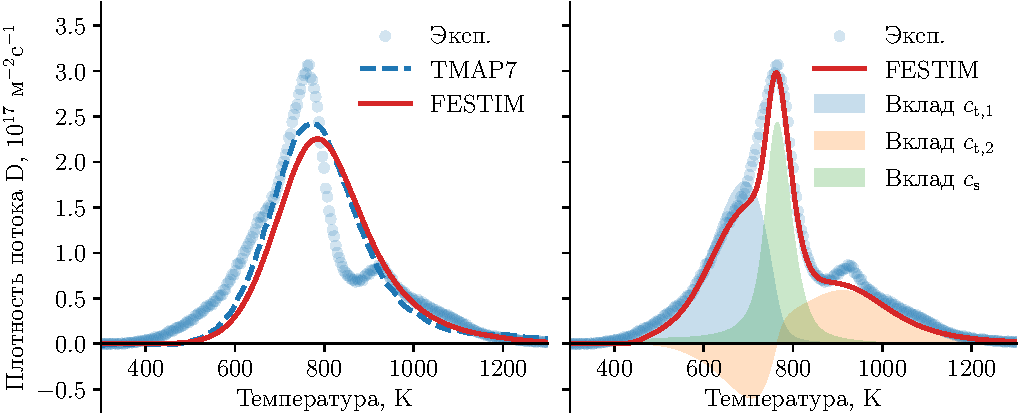
\includegraphics[scale=0.9]{QSPA_TDS.pdf}
	}
	\caption{Сравнение ТДС-спектров дейтерия из вольфрама, рассчитанных в коде FESTIM при двух предположениях о протекании процессов на поверхности, с данными, полученными в эксперименте и рассчитанными ранее в коде TMAP7~\cite{Poskakalov2020}. Вклад от различных сортов атомов определяется на основе изменения соответствующего интегрального содержания}\label{fig:QSPA_TDS}
\end{figure}

Раздел 3.2 посвящен численному моделированию накопления дейтерия в вольфраме под действием импульсно-периодических нагрузок, соответствующих ELM-событиям в крупных установках масштаба ИТЭР~\cite{Kulagin2025_JNM}. Задача рассматривалась в одномерном приближении для упрощенной геометрической модели, состоящей из трех материалов (вольфрама, меди, сплава бронзы) и соответствующей кратчайшему расстоянию между облучаемой и охлаждаемой поверхностями диверторных моноблоков ИТЭР (см. рисунок~\cref{fig:ITER_monoblock}). 

\begin{figure}[ht]
	\centering
	\begin{overpic}[scale=0.9]
		{ITER_monoblock.pdf}
		%\put(6, 75){ \textbf{(а)}}
		%\put(56.5, 75){ \textbf{(б)}}
		\put(74.2, 61.2){ $S_{\mathrm{ELM}}$}
		\put(71.2, 65.2){ $S_{\mathrm{stat}}$}
		\put(24.7, 77.4){$q_{\mathrm{heat}}$}
		\put(74.0, 77.4){$q_{\mathrm{heat}}$}
		\put(74.0, 5.2){$q_{\mathrm{loss}}$}
		\put(58.3, 40.4){$x$}
	\end{overpic}
	\caption{Полоидальное сечение диверторного моноблока ИТЭР (слева) и одномерное представление кратчайшего расстояния от облучаемой до водоохлаждаемой поверхности, соответствующее красной линии на левом рисунке. Размеры указаны в мм. \cruleme[customgrey]{0.5cm}{0.5cm}~---~W; \cruleme[customorange]{0.5cm}{0.5cm} "--- Cu; \cruleme[customyellow]{0.5cm}{0.5cm} "--- CuCrZr. }\label{fig:ITER_monoblock}
\end{figure}
В задаче транспорта дейтерия учитывались два источника подвижных атомов и один тип центров захвата, равномерно распределённый в объеме вольфрама. В части расчетов параметры центров захвата варьировались для оценки их влияния на интегральное накопление. В качестве базового случая были использованы следующие параметры: \( E_\mathrm{dt}=\SI{1.5}{\electronvolt} \); \( n_\mathrm{t}=\SI{1}{\text{ат.}\percent}\).

Моделирование проводилось для трех сценариев облучения, характеризуемых стационарными нагрузками с плотностью мощности 1, 5 и \SI{10}{\mega\watt\per\meter\squared}. Параметры облучения были выбраны в соответствии с результатами моделирования диверторной плазмы ITER в коде SOLPS~\cite{Pitts2025} при \( Q_\mathrm{fus}=10 \) (отношением произведённой энергии за счет реакции термоядерного синтеза к вложенной). Определение параметров потоков тепла и частиц проводилось на основе модели <<свободного потока>> (Free streaming model)~\cite{Fundamenski2006,Moulton2013}. Указанная модель позволяет получить аналитические выражения для временных зависимостей импульсных нагрузок, соответствующих экспериментально наблюдаемым зависимостям во время ELM-событий первого типа, и существенно снизить вычислительную сложность задачи. Выражения для плотности теплового потока (\( q_{\mathrm{ELM}} \)) и потока частиц (\(\Gamma_{\mathrm{ELM}} \)) во время ELM-событий представлены в следующем виде:
\begin{subequations}
	\label{eq:ch3/elm_fluxes}
	\begin{align}
		\frac{q_{\mathrm{ELM}}(t)}{q_{\mathrm{ELM,0}}}           & =\left(1+\left(\frac{\tau}{t}\right)^2\right)\left(\frac{\tau}{t}\right)^2\exp\left(-\left(\frac{\tau}{t}\right)^2\right),\label{eq:elm_heat_flux} \\
		\frac{\Gamma_{\mathrm{ELM}}(t)}{\Gamma_{\mathrm{ELM,0}}} & =\left(\frac{\tau}{t}\right)^2\exp\left(-\left(\frac{\tau}{t}\right)^2\right), \label{eq:elm_part_flux}
	\end{align}
\end{subequations}
где $\tau$ "--- постоянная времени, характеризующая фазу нарастания импульса~\cite{Eich2017}. 

Нормировка теплового потока проводилась на основе эмпирических выражений для плотности потока энергии плазменных нагрузок во время ELM-событий, полученных на основе обработки экспериментальных данных с внешней мишени действующих токамаков~\cite{Eich2017,VandenKerkhof2021}. В моделировании полагалось, что импульсные потоки тепла и частиц приходят в ту же область, что и стационарные потоки, а все использованные выражения справедливы для ELM-событий с характерной частотой повторения от 10 до \SI{100}{\hertz} (полная плотность энергии от \num{0.45} до \SI{0.14}{\mega\joule\per\meter\squared}). Сравнение потоков тепла и частиц при стационарном и импульсном воздействии приведено на рисунке~\cref{fig:ELM_fluxes}. 

\begin{figure}[ht]
	\centerfloat{
		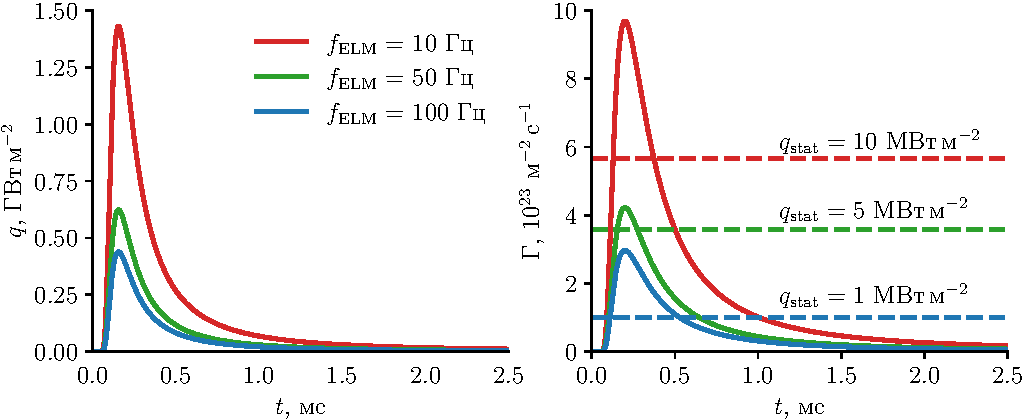
\includegraphics[scale=0.9]{ELM_fluxes.pdf}
	}
	\caption{Временные зависимости плотности потоков тепла (слева) и частиц (справа) во время ELM-событий при различных частотах повторения. Пунктирные линии соответствуют плотности потока частиц при стационарном облучении}\label{fig:ELM_fluxes}
\end{figure}

\begin{figure}[ht]
	\centerfloat{
		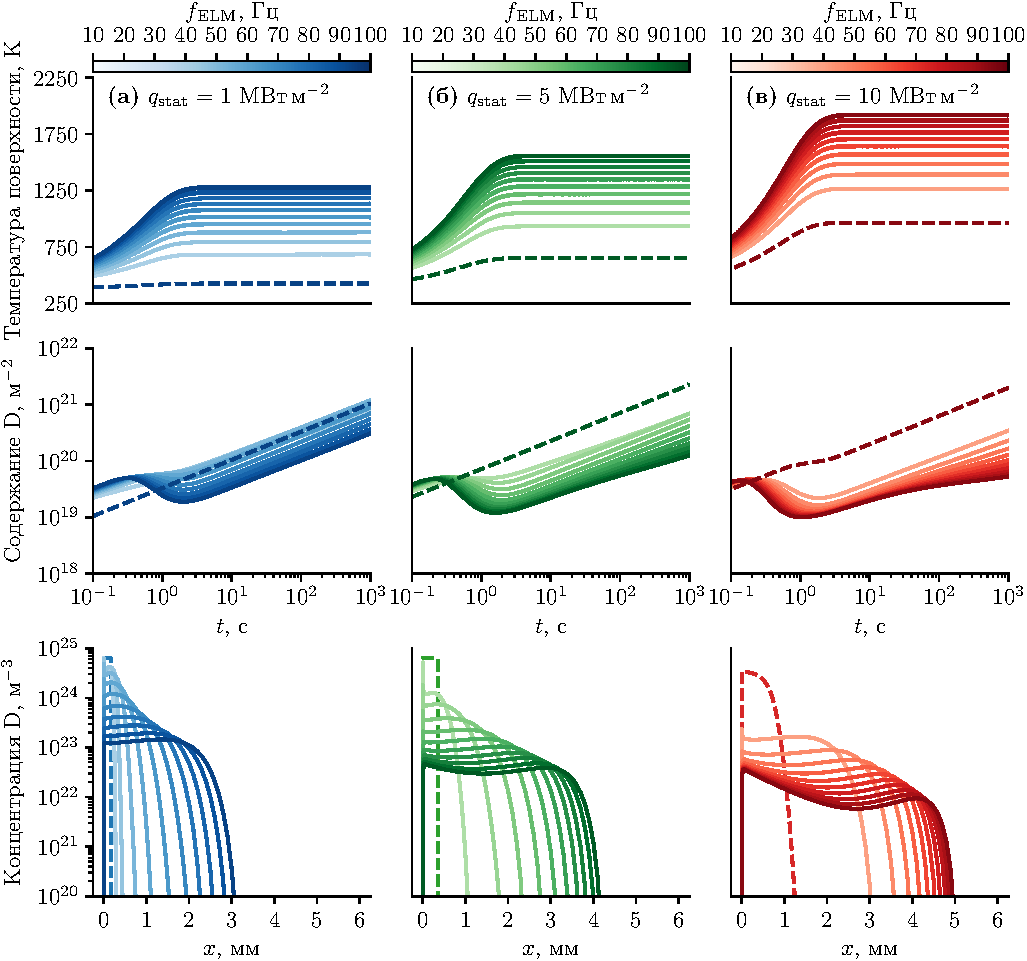
\includegraphics[scale=0.9]{ELMs_frequency.pdf}
	}
	\caption{Временные зависимости усредненной по длительности ELM-событий температуры поверхности (верхний ряд) и содержания дейтерия (средний ряд) при различных стационарных нагрузках. Пунктирные линии показывают соответствующие зависимости в случае без ELM-событий. Нижний ряд демонстрирует распределения концентрации дейтерия по глубине на последнем временном шаге}\label{fig:ELMs_frequency}
\end{figure}

В подразделе 3.2.3 показано, что при совместном воздействии стационарных и импульсно-периодических нагрузок температура материала выходит на квазиплато за время порядка нескольких секунд. Амплитуда осцилляций температуры поверхности увеличивается с уменьшением частоты повторения ELM-событий, когда ее среднее значение уменьшается. Из анализа динамики изменения профиля температуры следует, что флуктуации при достижении квазистационарного режима ограничены областью вольфрама. Это наблюдение было использовано далее в работе для редукции геометрической области, в которой решалась задача транспорта дейтерия. Сохранение эволюции профиля температуры достигалось за счет параметризации зависимости потока тепла, протекающего через границу раздела вольфрам-медь. Модельное время расчета было ограничено \SI{1000}{\second} для избежания достижения дейтерием границы раздела материалов.

Далее в работе проводится анализ влияния параметров облучения, центров захвата и скорости рекомбинации на поверхность для всех сценариев моделирования. В большинстве случаев было обнаружено снижение скорости накопления дейтерия во время переходных процессов. Характерные временные зависимости интегрального содержания при различных параметрах облучения приведены на среднем ряду рисунка~\cref{fig:ELMs_frequency}. Данное снижение вызвано существенным повышением температуры материала относительно базовых сценариев облучения без ELM-событий. Снижение зависит от соотношения стационарных и импульсно-периодических нагрузок и увеличивается с ростом частоты повторения ELM-событий. Из детального анализа влияния параметров моделирования были определены факторы, способные повысить скорость накопления во время ELM-событий. Наиболее значимые факторы включают наличие центров захвата с большим (\( >\SI{1.5}{\electronvolt} \)) барьером выхода, приводящим к захвату большей доли атомов, и присутствие барьера рекомбинации (\( >\SI{0.63}{\electronvolt} \)) на поверхности, ограничивающих десорбцию дейтерия.

С другой стороны, нагрев материала до высоких температур во время переходных процессов обеспечивает условия для более быстрой диффузии в объем (см. нижний ряд графиков на рисунке~\cref{fig:ELMs_frequency}), что может влиять на время проникновения изотопов водорода (включая радиоактивный тритий) в систему охлаждения ОПЭ и на эффективность последующего обезгаживания между экспериментальными кампаниями. Для демонстрации снижения эффективности обезгаживания была проведена отдельная серия расчетов, включающая три: облучение длительностью \SI{100}{\second}; простой и охлаждение материала длительностью \SI{1}{\hour}; обезгаживание материала при постоянной температуре \SI{513}{\kelvin} длительностью \SI{25}{\day}. На рисунке~\cref{fig:baking_efficiency} приведены значения эффективности обезгаживания при различных параметрах облучения.

\begin{figure}[ht]
	\centerfloat{
		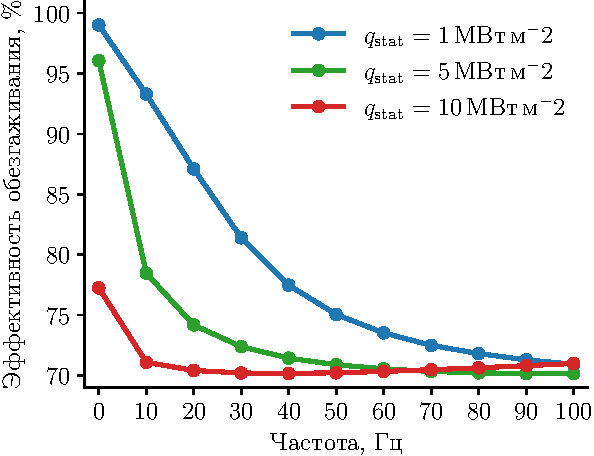
\includegraphics[scale=0.9]{baking_efficiency.pdf}
	}
	\caption{Зависимость эффективности обезгаживания от частоты ELM-событий в трех модельных сценариях облучения. Значения при нулевой частоте соответствуют случаю облучения только стационарными потоками тепла и частиц}\label{fig:baking_efficiency}
\end{figure}
Видно, что наибольшая эффективность достигается в случае только стационарного облучения. С увеличением фоновой нагрузки и частоты ELM-событий эффективность уменьшается, что вызвано проникновением дейтерия на большую глубину при нагреве материала до более высоких температур. На основе полученных результатов можно заключить, что протекание переходных процессов может влиять как на скорость накопления изотопов водорода во время плазменных разрядов, так и на эволюцию их содержания в ОПЭ во время иных этапов эксплуатации установки.  

В разделе 3.3 анализируется применимость использования усредненных по длительности ELM-событий потоков тепла и частиц для оценки средней величины интегрального накопления. Показано, что данный подход может воспроизводить результаты моделирования с учетом полной временной зависимости нагрузок, когда индуцированные колебания температуры и содержания дейтерия оказываются малы относительно средних значений. В рамках подхода данные условия выполняются при больших частотах повторения ELM-событий, соответствующих малым амплитудам флуктуаций нагрузок. Использование только стационарных компонент позволяет снизить вычислительную сложность задачи и рассмотреть квазистационарное приближение задачи для определения квазистационарных компонент температуры и концентраций~\cite{Marenkov2012a}.

В рамках квазистационарного приближения была рассмотрена задача транспорта дейтерия в вольфраме при учете влияния центров захвата и градиента температуры. Для упрощения математической постановки задачи было использовано приближение точечных источников подвижных атомов дейтерия с заданием нулевой концентрации атомов на левой границе и нулевой концентрации (гр. усл. Дирихле) или нулевого потока (гр. усл. Неймана) на правой. Показано, что при такой постановке задачи с помощью теоремы о суперпозиции и функции Грина краевой задачи возможно получить аналитические выражения, определяющие распределение стационарных компонент концентраций подвижных и неподвижных атомов дейтерия в материале, Учитывая использованную в работе функциональную зависимость теплоты переноса от температуры ($Q^*(T)=-\num{0.0045}\kBT^2$) были получены следующие выражения:
\begin{subequations}
	\begin{gather}
	\label{eq:ss_solution}
	\begin{array}{ll}
		\overline{c}_{\mathrm{m}}=&\exp\left(-Hx\right)\times
			\begin{cases}
			C_1(x,X_{\mathrm{stat}})+C_1(x,X_{\mathrm{ELM}}), & x \in [0,X_{\mathrm{stat}}],\\
			C_2(x,X_{\mathrm{stat}})+C_1(x,X_{\mathrm{ELM}}), & x \in [X_{\mathrm{stat}},X_{\mathrm{ELM}}],\\
			C_2(x,X_{\mathrm{stat}})+C_2(x,X_{\mathrm{ELM}}), & x\in [X_{\mathrm{ELM}}, L],
			\end{cases}
	\end{array}\\
    \overline{c}_{\mathrm{t}}=\dfrac{n_{\mathrm{t}}}{1+\dfrac{n_{\mathrm{t}}\nu_{\mathrm{dt}}(\overline{T})}{\overline{c}_{\mathrm{m}}\nu_{\mathrm{t}}(\overline{T})}}, \\
	C_1(x,X_i)=\Gamma_i^{\mathrm{imp}}G_1(x,X_i),\\
	C_2(x,X_i)=\Gamma_i^{\mathrm{imp}}G_2(x,X_i),
	\end{gather}
\end{subequations}
где \( \Gamma_i^{\mathrm{imp}} \) "--- плотность потока имплантированных атомов, \si{\per\meter\squared\per\second}; \( X_i \) "--- характерная глубина внедрения атомов, \si{\meter}; индекс \( i \) соответствует стационарным (<<stat>>) или импульсно-периодическим (<<ELM>>) нагрузкам. 

Функция Грина определяется в зависимости от условия на правой границе и профиля температуры. В общем виде она выражается следующим образом:
\begin{subequations}
	\begin{align}
		 & \text{Если гр. усл. Дирихле}:
		\begin{cases}
			G_1(x,y)=\int\limits_0^x\dfrac{d\chi}{p(\chi)}\,\dfrac{\int\limits_y^L\dfrac{d\chi}{p(\chi)}}{\int\limits_0^L\dfrac{d\chi}{p(\chi)}}, & x\in[0,y], \\[25pt]
			G_2(x,y)=\int\limits_0^y\dfrac{d\chi}{p(\chi)}\,\dfrac{\int\limits_x^L\dfrac{d\chi}{p(\chi)}}{\int\limits_0^L\dfrac{d\chi}{p(\chi)}}, & x\in[y,L]. \\
		\end{cases} \\[10pt]
		 & \text{Если гр. усл. Неймана}:
		\begin{cases}
			G_1(x,y)=\int\limits_0^x\dfrac{d\chi}{p(\chi)}, & x\in[0,y], \\[10pt]
			G_2(x,y)=\int\limits_0^y\dfrac{d\chi}{p(\chi)}, & x\in[y,L].
		\end{cases}
	\end{align}
\end{subequations}
где $p(x)=D(\overline{T})\exp\left(-\int\limits_0^x H(\overline{T})d\chi\right)$; $H(\overline{T})=Q^*(\overline{T})\partial_x \overline{T}/k\overline{T}^2$. 

На рисунке~\cref{fig:retention_saturation} показано сравнение аналитических профилей концентрации с рассчитанными численно для трех сценариев при различных параметрах облучения и свойствах центров захвата. Расчетные профили концентрации при средних компонентах нагрузок были получены с гауссовым распределением источников внедренных атомов. Моделирование проводилось до достижения насыщения. Из сравнения видно, что аналитические профили хорошо коррелируют с полученными на основе численного расчета профилями при различных комбинациях входных параметров, но представляют собой незначительно заниженную оценку, так как не учитывают протяженность профиля внедренных частиц. Также можно заметить, что наибольшее содержание дейтерия при насыщении достигается вблизи правой границы, где температура материала наименьшая.
\begin{figure}[ht]
	\centerfloat{
		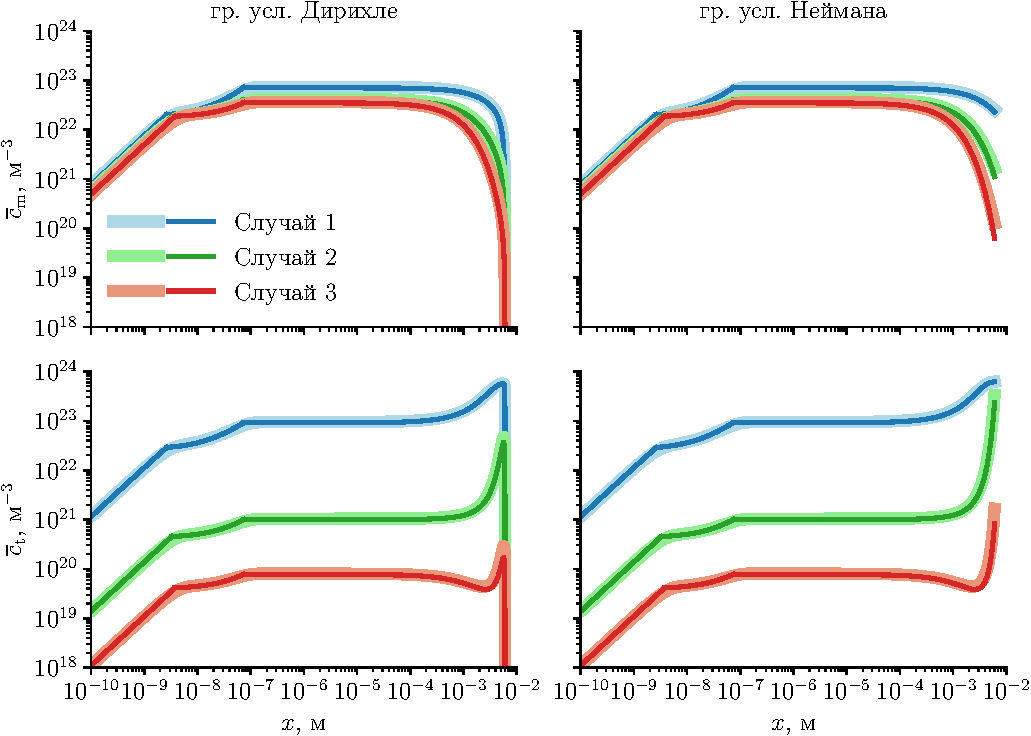
\includegraphics[scale=0.9]{retention_saturation.pdf}
	}
	\caption{Сравнение аналитических профилей концентрации дейтерия при насыщении (тонкие линии) с профилями, полученными на основе численных расчетов с использованием средних компонент потоков тепла и частиц (широкие линии)}\label{fig:retention_saturation}
\end{figure}

В \underline{\textbf{четвёртой главе}} представлены результаты численного моделирования десорбции дейтерия из вольфрама при импульсном лазерном воздействии. Раздел 4.1 посвящен валидации расчетной модели на основе экспериментальных данных по ЛИД дейтерия из пленок вольфрама (\SI{1}{\micro\meter}), соосажденных на медные подложки (толщина \SI{3}{\milli\meter}). Эксперименты проводились научным коллективом ФТИ им. А.Ф. Иоффе при непосредственном участии автора. 

Для обеспечения лучшего теплоотвода во время ЛИД образцы укладывались на дополнительное медное основание толщиной \SI{3}{\milli\meter}, между медными элементами устанавливались индиевые прокладки. Были использованы две длительности лазерных импульсов \SI{220}{\micro\second} и \SI{1}{\milli\second} (оптоволоконная лазерная система, IPG YLR-2000, \SI{1070}{\nano\metre}) с прямоугольным временным профилем и гауссовым пространственным распределением (ширина профиля \SI{1}{\milli\meter}). Полная энергия лазерных импульсов варьировалась в ходе экспериментов и была ограничена достижением температуры плавления меди. 

Измерения при фиксированной длительности лазерного пучка проводились на отдельных образцах. Участки поверхности образцов облучались серией импульсов с частотой \SI{0.1}{\hertz}. Регистрация сигналов 2; 3 и 4 масс осуществлялась с помощью квадруполного масс-спектрометра (Extorr XT300M). Масс-спектрометр калибровался по постоянному потоку дейтериевой течи с уровнем потока \SI{e-6}{\metre\cubed\pascal\per\second}. В ходе экспериментов изменения в сигналах 3 и 4 масс были ярко выражены, когда сигнал 2-ой массы не отличался от фонового. По временным зависимостям потоков частиц были определены значения полного числа десорбированных атомов дейтерия. Получение дополнительной информации о параметрах центров захвата в осажденных пленках осуществлялось методом ТДС. Были исследованы аналогичные образцы с соосажденными пленками толщиной \SI{0.5}{\micro\metre}. Измерения проводились на сверхвысоковакуумном стенде \thesisOrganizationShort / (кафедра №21)~\cite{Rusinov2009} с постоянной скоростью нагрева \SI{0.5}{\kelvin\per\second}.

Анализ ТДС-спектра проводился на основе численного моделирования в одномерном приближении. Было установлено, что воспроизвести спектр возможно при предположении наличия четырех типов центров захвата:
\begin{enumerate}[beginpenalty=10000]
    \item \( n_\mathrm{t,1}=\SI{2.89}{\text{ат.}\percent} \), \( E_\mathrm{dt,1}=\SI{1.108}{\electronvolt} \);
    \item \( n_\mathrm{t,2}=\SI{1.79}{\text{ат.}\percent} \), \( E_\mathrm{dt,2}=\SI{1.279}{\electronvolt} \);
    \item \( n_\mathrm{t,3}=\SI{1.97}{\text{ат.}\percent} \), \( E_\mathrm{dt,3}=\SI{1.536}{\electronvolt} \);
    \item \( n_\mathrm{t,4}=\SI{0.60}{\text{ат.}\percent} \), \( E_\mathrm{dt,4}=\SI{1.818}{\electronvolt} \).
\end{enumerate}
Оцененное содержание дейтерия в пленках составляет более 7 ат.\%. Из сравнения с литературными источниками следует, что значения барьеров выхода в диапазоне \SIrange{1.0}{1.5}{\electronvolt} могут соответствовать вакансиям в решетке вольфрама, занятыми одним (\(\approx\SI{1.5}{\electronvolt}\)) или несколькими атомами дейтерия (\(<\SI{1.5}{\electronvolt}\)), когда центр захвата с наибольшим барьером выхода (тип 4) может соответствовать выходу дейтерия из вакансионного кластера. 

На основе полученных данных о параметрах центров захвата было проведено моделирование ЛИД. С целью воспроизведения результатов экспериментальных измерений была рассмотрена упрощенная геометрическая модель в цилиндрических координатах с аксиальной симметрией, состоящая из двух материалов: вольфрамовой пленки толщиной \SI{1}{\micro\meter} и медной подложки толщиной \SI{6}{\milli\meter}. Лазерный нагрев задавался в качестве потока тепла на поверхности с параметрами облучения, соответствующими экспериментальным данным. Для сравнения были выбраны результаты, полученные только после первых выстрелов из каждой серии импульсов при различных энергиях пучка. В разделе отмечается, что в экспериментах не было возможности контролировать температуру поверхности, что не позволило убедиться в точности полученного решения уравнения теплопроводности. В частности, отсутствовала информация о коэффициенте поглощения лазерного излучения (\( A \)). Для учета указанной неопределенности коэффициент поглощения лазерного излучения расценивался как свободный.

Сравнение результатов моделирования и экспериментальных измерений представлено на рисунке~\cref{fig:LID_Comparison}, где приведены зависимости интегрального числа десорбированных атомов от полной энергии лазерного импульса. Результаты моделирования демонстрируют хорошее согласие с экспериментальными данными при значении коэффициента поглощения лазерного излучения \(A=\num{0.55}\). Для демонстрации влияния коэффициента поглощения на рисунке также приведена область изменения результатов при варьировании параметра от \num{0.5} до \num{0.6}. Из сравнения результатов следует, что применение более длительных импульсов позволяет проводить анализ в более широком диапазоне температур ввиду меньше скорости нагрева. Число атомов десорбированного дейтерия оказывается выше при предельной тепловой нагрузке в случае использования миллисекундного ЛИД, что демонстрирует влияние длительности лазерного нагрева на эффективность анализа. Повышение точности измерений параметров нагрева и температурного профиля пленки при ЛИД позволит уточнить решение задачи теплопереноса. Несмотря на имеющиеся неопределенности, наблюдается хорошее согласие между экспериментальными результатами и расчетами, выполненными в рамках стандартной модели транспорта изотопов водорода.

\begin{figure}[ht]
    \centerfloat{
        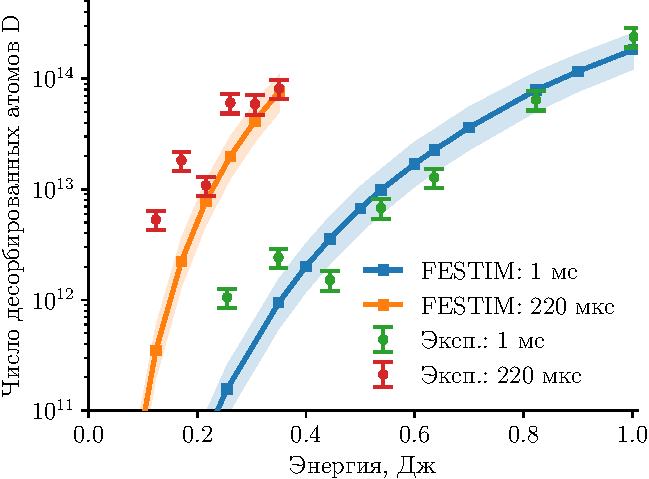
\includegraphics[scale=0.9]{LID_Comparison.pdf}
    }
    \caption{Сравнение расчетных и экспериментальных зависимостей числа десорбированных частиц от энергии лазерного импульса. Сплошные линии соответствуют коэффициенту поглощения излучения \( A=\num{0.55} \), закрашенные области "--- \( A = \SIrange{0.5}{0.6}{} \)}\label{fig:LID_Comparison}
\end{figure}

В разделах 4.2 "--- 4.3 приведены результаты комплексного исследования влияния параметров лазерного облучения, процессов на поверхности, параметров материала и центров захвата. Исследование было проведено в рамках одномерного приближения при учете одного типа центров захвата в приповерхностном слое толщиной \SI{10}{\micro\meter}. Рассматривались три сценария нагрева лазерными импульсами с различными временными профилями, соответствующими экспериментальным лазерным системам: наносекундный нагрев с гауссовым распределением (ширина \SI{25}{\nano\second}), микросекундный нагрев с прямоугольным профилем (длительность \SI{10}{\micro\second}) и миллисекундный нагрев с трапециевидным профилем (длительность \SI{5}{\milli\second}). Предельное значение плотности поглощенной энергии выбиралось таким образом, чтобы максимальная температура в ходе нагрева не достигала точки плавления вольфрама.

В подразделе 4.2.2 проводится анализ состава потока десорбированных частиц для оценки величины атомарной фракции (отношение числа десорбированных напрямую атомов к полному числу вышедших атомов). Как отмечается, информация о величине атомарной фракции может быть необходима для точной интерпретации результатов экспериментальных измерений при определении содержания изотопов водорода методом ЛИД. Для оценки величины атомарной фракции была рассмотрена совокупность каналов десорбции молекул, содержащих атомы с поверхности и из приповерхностной области, и прямой десорбции атомов с поверхности~\cite{Pisarev1997}. 

В приближении локального равновесия процессов вблизи поверхности были получены аналитические выражения, определяющие зависимости степени покрытия поверхности (\( \theta \)) и атомарной фракции (\( f_\mathrm{a} \)) от температуры и плотности полного потока десорбированных атомов~\cite{Kulagin2022a_rus}. В безразмерной форме полученные выражения имеют следующее представление:
\begin{subequations}
    \begin{align}
        \theta       & = \frac{\kas}{4 \kms} \left( \sqrt{1+\dfrac{8j_\mathrm{des}\kms}{(\kas)^2}} -1 \right),               \\
        f_\mathrm{a} & = \frac{(\kas)^2}{4 j_\mathrm{des} \kms} \left( \sqrt{1+\dfrac{8j_\mathrm{des}\kms}{(\kas)^2}} -1 \right),
    \end{align}
\end{subequations}
где \( \kas \) "--- безразмерная константа скорости прямой десорбции атомов с поверхности; \( \kms \) "--- безразмерная константа скорости десорбции молекул с поверхности; \( j_\mathrm{des} \) "--- безразмерная плотность полного поток атомов. Данные выражения были получены без учета возможного насыщения поверхности и влияния десорбции молекул, содержащих атомы из приповерхностной области.

На основе полученных выражений была построена диаграмма значений атомарной фракции в зависимости от температуры поверхности и полного потока десорбированных частиц, приведенная на рисунке~\cref{fig:atomic_fraction_diagram}. Область применимости ограничена изолинией \(\theta=1\), показанной белой пунктирной линией на рисунке. Тем не менее, диаграмма остается в целом корректной, так как в области правее изолинии будет доминировать десорбция молекул. Из диаграммы следует, что десорбция молекул является доминирующим механизмом десорбции при высокой плотности выходящих частиц. Атомарная фракция становится значимой только при сравнительно высоких температурах поверхности. Однако такие температуры вполне могут быть достигнуты при лазерном нагреве поверхности для обеспечения наибольшей эффективности ЛИД. 

\begin{figure}[ht]
    \centerfloat{
        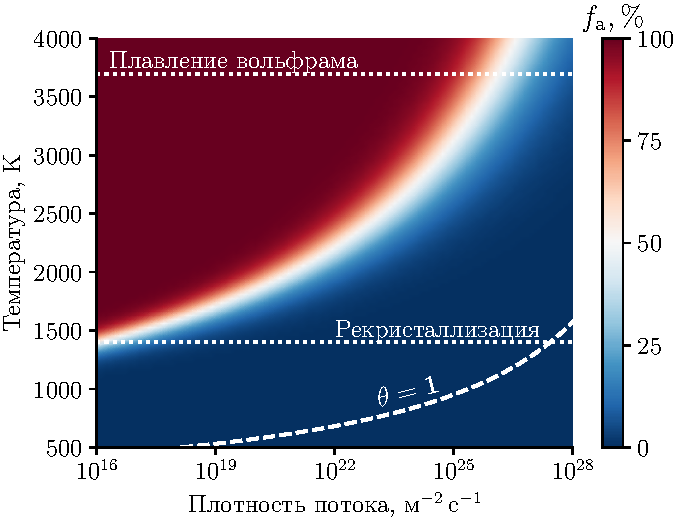
\includegraphics[scale=0.9]{atomic_fraction_diagram.pdf}
    }
    \caption{Атомарная фракция в приближении равновесия процессов у поверхности при различных значениях температуры и плотности полного потока десорбированных частиц}\label{fig:atomic_fraction_diagram}
\end{figure}

Результаты численных расчетов~\cite{Kulagin2022b}, представленные в подразделе 4.2.3, подтверждают качественный анализ. Значимый интегральный вклад от прямой десорбции атомов ($\sim\SI{10}{\percent}$) наблюдается исключительно при длительном (>\SI{10}{\micro\second}) нагреве поверхности до высоких температур ($\max(T)>\SI{2500}{\kelvin}$). Нагрев поверхности коротким импульсом с наносекундной длительностью инициирует выход дейтерия с большой плотностью потока, что приводит к преимущественной десорбции молекул с поверхности. Полученные результаты позволяют полагать, что увеличение концентрации центров захвата или уменьшение энергии связи приведет к снижению атомарной фракции в общем потоке десорбции. Также отмечается, что получение более точных оценок потребует проведения дополнительных исследований для минимизации неопределенности, связанной со значениями характерных параметров, определяющих вероятность десорбции за счет различных механизмов.

В разделе 4.3 приводится оценка эффективности ЛИД (отношение числа десорбированных атомов к их начальному количеству) в широком диапазоне параметров~\cite{Kulagin2023}. Отмечается, что в условиях экспериментальных установок анализируются поверхностные слои, физические свойства которых точно неизвестны (теплофизические свойства, концентрация и степень заполнения центров захвата, энергия связи атомов с ними), что может усложнять постобработку экспериментальных измерений. 

Рисунок~\cref{fig:LID_kappa_n_Edt_var} обобщает результаты проведенных расчетов. Для оценки влияния теплофизических свойств была проведено варьирование теплопроводности вольфрама при сохранения функциональной зависимости от температуры (\( \kappa \rightarrow a\kappa \)). Как показано в левой колонке рисунка~\cref{fig:LID_kappa_n_Edt_var} для наносекундной (верхний график) и миллисекундной (нижний график) длительностей, большая часть данных совпадает при низких температурах, но в высокотемпературной области наблюдается небольшой разброс. Закрашенные области соответствуют диапазону изменения эффективности при варьировании теплопроводности: коэффициент \(a\) увеличивается от нижней границы к верхней. Указанный разброс объясняется изменением распределения температуры в объеме. В целом, небольшое изменение свойств материала слабо влияет на результаты, поскольку десорбция дейтерия в основном определяется выходом атомов из наиболее нагретой приповерхностной области. Аналогичные рассуждения можно провести для удельной теплоемкости материала: с уменьшением теплоемкости ожидается снижение эффективности десорбции при фиксированной температуре из-за уменьшения характерной глубины проникновения тепла.

\begin{figure}[ht]
    \centerfloat{
        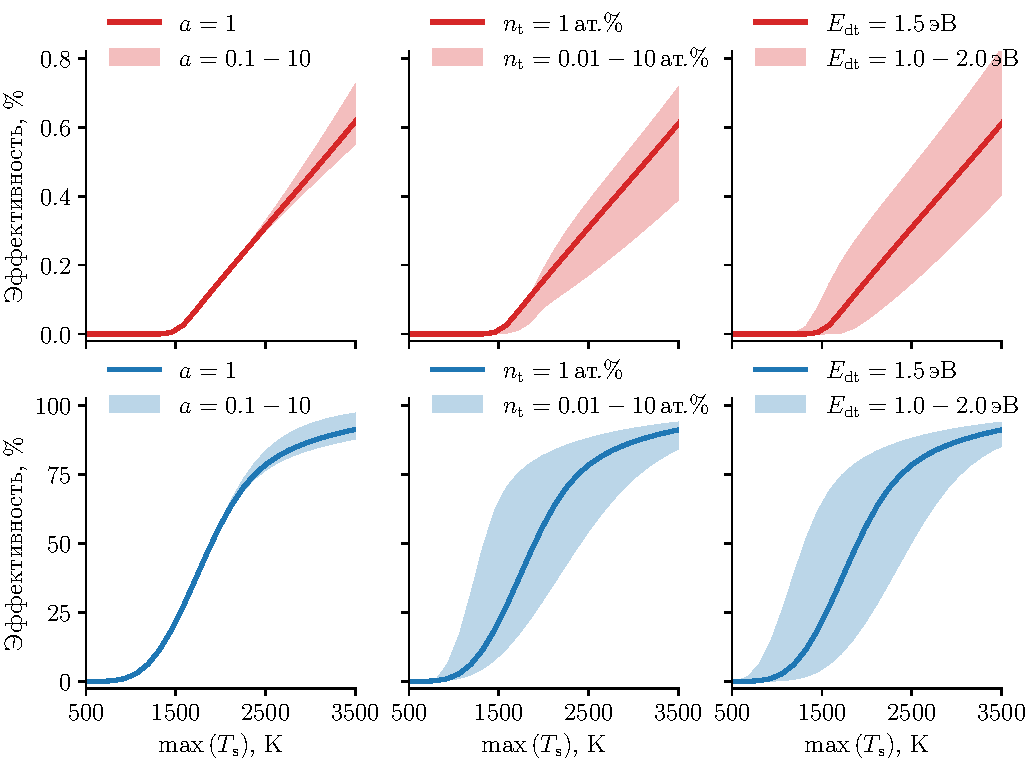
\includegraphics[scale=0.9]{LID_kappa_n_Edt_var.pdf}
    }
    \caption{Зависимости эффективности ЛИД от максимальной температуры поверхности при различных значениях теплопроводности (слева), при различных концентрациях центров захвата (по середине) и при различных барьерах выхода из центров захвата (справа). Верхние графики соответствуют наносекундному нагреву, нижние "--- миллисекундному. Сплошные линии указывают зависимости, рассчитанные при базовой комбинации параметров}\label{fig:LID_kappa_n_Edt_var}
\end{figure}

Влияние параметров центров захвата показано в центральном и правом рядах рисунка. Десорбция оказывается более эффективной в случае дефектов с низким барьером выхода и низкой концентрацией в широком температурном диапазоне (оба параметра на графиках увеличиваются от верхней границы закрашенной области к нижней). Изменение свойств центров захвата влияет на скорость роста эффективности и, как следствие, на пороговое значение температуры, при которой инициируется десорбция. Таким образом, максимальный разброс значений для всех сценариев нагрева наблюдается при низких температурах и уменьшается для более горячих режимов. Стоит заметить, что совпадение эффективностей ЛИД при различных комбинациях (\(n_\mathrm{t}, E_\mathrm{dt}\)) соответствует разному числу десорбированных атомов дейтерия, демонстрируя универсальность параметра эффективности. 

Важным наблюдением является то, что лишь изменение концентрации центров захвата на несколько порядков способно вызвать сопоставимое изменение эффективности ЛИД, как при увеличении барьера выхода. Очевидно, что влияние концентрации ловушек менее выражено, поскольку вероятность выйти из дефекта экспоненциально зависит от энергетического барьера перехода. Отдельного внимания заслуживают данные, полученные для случая миллисекундного нагрева (синие зависимости). Они показывают, что использование более длительных тепловых импульсов повышает эффективность обезгаживания поверхностного слоя. Однако также видно, что 100\%-ная эффективность десорбции из толстого слоя, вероятно, не может быть достигнута за один импульс. В работе показано, что достижение предельной эффективности выхода может определяться диффузией дейтерия за пределы области удержания, тогда как нижний определяется присутствием центров захвата большим барьером выхода и высокой концентрацией. Эти ограничивающие факторы указывают на необходимость увеличения длительности нагрева или проведения многократного облучения поверхности для достижения полного выхода захваченных атомов.

В работе также было продемонстрировано, что в зависимости от длительности лазерного импульса десорбция атомов может определяться как процессами на поверхности (в случае наносекундного нагрева), так и процессами в объеме (в случае микросекундной длительности и более). В конце работы проводится качественный анализ режимов десорбции во время ЛИД. Показано, что дифференцировать режимы можно на основе безразмерного параметра \( \xi=\tau_\mathrm{D}/\tau_\mathrm{des} \), описывающего отношение характерного времени диффузионного переноса к характерному времени десорбции с поверхности. 

В приближении доминирующего влияния механизмов десорбции с участием адсорбированных атомов была предложена оценка характерного времени десорбции:
\begin{equation}
    \tau_\mathrm{des}^{-1} \sim \dfrac{\nu_\mathrm{a}^\mathrm{s}}{2} \left( 1 + \sqrt{1+\dfrac{8J_\mathrm{des}\nu_\mathrm{m}^\mathrm{s}}{(\nu_\mathrm{a}^\mathrm{s})^2}} \right),
\end{equation}
где \( \nu_\mathrm{a}^\mathrm{s} \) "--- константа скорости прямой десорбции атомов с поверхности, \si{\second}; \( \nu_\mathrm{m}^\mathrm{s} \) "--- константа скорости десорбции атомов в составе молекул с поверхности, \si{\meter\squared\per\second}; \( J_\mathrm{des} \) "--- полный поток десорбированных частиц, \si{\per\meter\squared\per\second}. Характерное время диффузионного переноса с учетом влияния центров захвата оценивается на основе эффективного коэффициента диффузии:
\begin{subequations}
    \begin{align}
        \tau_\mathrm{D}         & \sim \frac{\delta_\mathrm{eff}^2}{D_\mathrm{eff}}, \\
        D_\mathrm{eff} & = \dfrac{D}{1+\dfrac{n_\mathrm{t}\nu_\mathrm{t}}{\nu_\mathrm{dt}}}. 
    \end{align}
\end{subequations}
В случае малого градиента температуры в приповерхностной области эффективная длина диффузии оценивается как: \( \delta_\mathrm{eff} \sim \sqrt{\int\limits_0^t D_\mathrm{eff}(T_\mathrm{s})dt'}\). 

Десорбция ограничена процессами в объеме, когда \( \xi \gg 1 \), и определяется процессами на поверхности, когда \( \xi \ll 1 \). Таким образом, выход изотопов водорода за весь лазерный импульс можно считать ограниченными объемными процессами, если преобладающая часть атомов десорбируется при \( \xi \gg 1 \). На основе сравнения с результатами численного моделирования показано, что такой качественный подход может быть использован для определения режима ЛИД. Наибольший интерес вызывает случай, когда выход изотопов водорода определяется процессами в объеме. В этом случае задачу ЛИД можно упростить, сведя её к рассмотрению только транспорта дейтерия без учета кинетики процессов на поверхности, что предоставляет определённые преимущества при интерпретации результатов экспериментальных измерении.

\FloatBarrier
\pdfbookmark{Заключение}{conclusion}                                  % Закладка pdf
В \underline{\textbf{заключении}} приведены основные результаты работы, которые заключаются в следующем:
%% Согласно ГОСТ Р 7.0.11-2011:
%% 5.3.3 В заключении диссертации излагают итоги выполненного исследования, рекомендации, перспективы дальнейшей разработки темы.
%% 9.2.3 В заключении автореферата диссертации излагают итоги данного исследования, рекомендации и перспективы дальнейшей разработки темы.
В рамках данной диссертационной работы методом численного моделирования были исследованы закономерности захвата и десорбции дейтерия в вольфраме при импульсных плазменном и лазерном воздействии. Среди наиболее значимых результатов можно выделить следующие:
\begin{enumerate}
  \item В программном пакете FESTIM была реализована модель, учитывающая кинетику процессов на поверхности. Реализованная модель расширяет функциональные возможности кода, что подтверждено в ходе проверки корректности ее имплементации. Модель включена в состав свободно распространяемого программного обеспечения и доступна всем пользователям.
  \item Сравнение результатов моделирования с экспериментальными данными по захвату дейтерия в вольфраме при импульсном плазменном облучении и экспериментами по ЛИД дейтерия из вольфрамовых пленок показало хорошее соответствие, что подтверждает применимость стандартных моделей для анализа динамики транспорта дейтерия при импульсных нагрузках.
  \item На основе численного моделирования проведен комплексный анализ влияния импульсно-периодических плазменных нагрузок, соответствующих ELM-событиям в крупных токамаках, на долговременное накопление дейтерия в вольфраме. Установлено, что в широком диапазоне параметров облучения скорость накопления дейтерия в переходных процессах снижается вследствие существенного нагрева материала высокоэнергетичными частицами. Эффект усиливается с ростом частоты импульсных нагрузок. 
  \item Показано, что дополнительный нагрев во время переходных процессов способствует более глубокому проникновению дейтерия. Данный эффект усиливается с увеличением частоты импульсных нагрузок, приводящих к росту средней температуры материала. В условиях термоядерных установок это может влиять как на скорость проникновения изотопов водорода в систему охлаждения, так и на эффективность дегазации элементов установки между плазменными кампаниями.
  \item В приближении малых импульсных нагрузок во время переходных событий построена аналитическая модель, описывающая квазистационарное распределение дейтерия в материале с учетом влияния центров захвата и градиента температур. Развитая модель может быть использована для оценки предельного уровня содержания изотопов водорода в квазистационарном режиме при достижении насыщения.
  \item Проведен детальный численный анализ состава потока десорбированных частиц при ЛИД. Установлено, что вероятность прямой десорбции атомов увеличивается с ростом температуры поверхности и уменьшением полного потока выходящих частиц. Условия для десорбции атомов могут быть выполнены при использовании лазерных импульсов с длительностью от \SI{10}{\micro\second}. В рамках подхода получена оценка атомарной фракции на уровне \( \sim \SI{10}{\percent} \) в случае использования лазерных импульсов с миллисекундной длительностью, что может вносить дополнительную погрешность при проведении оценки содержания изотопов водорода.
  \item Исследована эффективность анализа содержания дейтерия методом ЛИД в широком диапазоне параметров материала и лазерного облучения. Наибольшая эффективность достигается при использовании более длительных лазерных импульсов. Показано, что измерение температуры поверхности позволяет снизить влияние неопределенности теплофизических свойств материала на точность измерений. Основным источником погрешности является неопределенность энергетического барьера выхода из центров захвата, тогда как влияние концентрации центров захвата оказывается менее значительным.    
\end{enumerate}


\pdfbookmark{Литература}{bibliography}                                % Закладка pdf
\ifdefmacro{\microtypesetup}{\microtypesetup{protrusion=false}}{} % не рекомендуется применять пакет микротипографики к автоматически генерируемому списку литературы
\urlstyle{rm}                               % ссылки URL обычным шрифтом
\ifnumequal{\value{bibliosel}}{0}{% Встроенная реализация с загрузкой файла через движок bibtex8
    \renewcommand{\bibname}{\large \bibtitleauthor}
    \nocite{*}
    \insertbiblioauthor           % Подключаем Bib-базы
    %\insertbiblioexternal   % !!! bibtex не умеет работать с несколькими библиографиями !!!
}{% Реализация пакетом biblatex через движок biber
    % Цитирования.
    %  * Порядок перечисления определяет порядок в библиографии (только внутри подраздела, если `\insertbiblioauthorgrouped`).
    %  * Если не соблюдать порядок "как для \printbibliography", нумерация в `\insertbiblioauthor` будет кривой.
    %  * Если цитировать каждый источник отдельной командой --- найти некоторые ошибки будет проще.
    %

    %
    %% authorscopus
    \nocite{Kulagin2022a_rus}%
    \nocite{Kulagin2022b}%
    \nocite{Kulagin2023}%
    % \nocite{Kulagin2024}%
    \nocite{Kulagin2025_JNM}%
    \nocite{Kulagin2025_IJHE}% 

    \ifnumgreater{\value{usefootcite}}{0}{
        \begin{refcontext}[labelprefix={}]
            \ifnum \value{bibgrouped}>0
                \insertbiblioauthorgrouped    % Вывод всех работ автора, сгруппированных по источникам
            \else
                \insertbiblioauthor      % Вывод всех работ автора
            \fi
        \end{refcontext}
    }{
        \ifnum \totvalue{citeexternal}>0
            \begin{refcontext}[labelprefix=A]
                \ifnum \value{bibgrouped}>0
                    \insertbiblioauthorgrouped    % Вывод всех работ автора, сгруппированных по источникам
                \else
                    \insertbiblioauthor      % Вывод всех работ автора
                \fi
            \end{refcontext}
        \else
            \ifnum \value{bibgrouped}>0
                \insertbiblioauthorgrouped    % Вывод всех работ автора, сгруппированных по источникам
            \else
                \insertbiblioauthor      % Вывод всех работ автора
            \fi
        \fi
        %  \insertbiblioauthorimportant  % Вывод наиболее значимых работ автора (определяется в файле characteristic во второй section)
        \begin{refcontext}[labelprefix={}]
            \insertbiblioexternal            % Вывод списка литературы, на которую ссылались в тексте автореферата
        \end{refcontext}
        % Невидимый библиографический список для подсчёта количества внешних публикаций
        % Используется, чтобы убрать приставку "А" у работ автора, если в автореферате нет
        % цитирований внешних источников.
        \printbibliography[heading=nobibheading, section=0, env=countexternal, keyword=biblioexternal, resetnumbers=true]%
    }
}
\ifdefmacro{\microtypesetup}{\microtypesetup{protrusion=true}}{}
\urlstyle{tt}                               % возвращаем установки шрифта ссылок URL
